\documentclass{article}

\usepackage{amsmath}
\usepackage{graphicx}

\newcommand{\grad}{\nabla}
\newcommand{\sign}{{\text{sign}}}
\newcommand*\rfrac[2]{{}^{#1}\!/_{#2}}

\begin{document}

\thispagestyle{empty}

\begin{center}
\bf\large
Final Report:\\
\Huge
HogWildChild!
\end{center}

\begin{center}
\large
Ryan Flood and Billy Wood\\
15-418 Final Project\\
Due: \today
\end{center}

\clearpage
\pagenumbering{roman}

\tableofcontents

\clearpage
\pagenumbering{arabic}

\section{Summary}

We implemented the HogWild! algorithm, as described in a paper
\cite{hogwild} from the 
University of Wisconsin-Madison, and further attempted to update the
algorithm for datasets where some variables occur frequently.
The algorithm is designed for performing stochastic gradient descent in
parallel.
We ran our code on the Intel Xeon 6-core CPUs in the GHC27-46 machines.
This is the same chip used in the original HogWild! paper, and our goal
was to match their results of 4x speedup.

\section{Background}

HogWild! is an algorithm for performing Stochastic Gradient Descent (SGD)
in parallel.
SGD is an optimization method for minimizing the error in a machine
learning algorithm.
Essentially, if you have some set of decision variables, $w$,
you can let $E(w)$ be the error on the training set using decision
variables $w$.
Gradient descent iteratively sets $w := w - \alpha \grad E(w)$,
where $\alpha$ is known as the learning rate and decreases with each
iteration of the algorithm (as you hone in on a sufficiently accurate
solution).
SGD approximates the true gradient of $E$ using the gradient at a single
data point, and sweeps through the entire training set, updating $w$
after each example.

This is where parallelization is desired.
Since each datapoint updates the decision variables,
and each datapoint uses the decision variables when computing the gradient,
it seems important that these changes be made serially.

The HogWild! paper gives conditions where it is okay to perform these
changes in parallel.
In particular, HogWild requires \emph{sparse separable cost functions}
of the form:
\[
    E(w) = \sum\limits_{d \in D} e_d(w_d)
\]
Where $d \in D$ denotes a small subset of the decision variables in $w$.
Essentially, the $d$ is a training example, which only depends on some
subset of the decision variables.
$e_d$ is the error associated with that particular training sample,
and so we can approximate the gradient of $E(w)$ at data point $d$
by $\grad e_d(w_d)$.

This provides the opportunity for a lot of data parallelism,
because if data samples $d_1$ and $d_2$ use different decision variables,
you can easily compute $\grad e_{d_1}(w)$ and $\grad e_{d_2}(w)$ in
parallel and apply these updates to $w$.

As we sought to investigate the parallelism of this approach, we chose
to focus on gradient descent in a Support Vector Machine (SVM).
SVM is an algorithm for classifying samples between two different
classes, represented by $\{-1, 1\}$.
For a data sample $z$, and decision variabels $w$, we can compute the
output of the svm as $\sign(w \cdot z)$.
In this, the error term over all the data is:
\[
    \min\limits_w \left(\sum\limits_{d\in D} \max(1-y_d w^T z_d, 0)\right)
                  + \lambda \|w\|^2
\]
Where $d = (z,y)$ is a data sample, with value $y \in \{-1, 1\}$.
The term $\lambda \|w\|^2$ is used to prioritize small values of $w$,
as these behave less eradically on new data.

This can be changed into a sparse separable function as described by:
\[
    \min\limits_w \sum\limits_{d \in D}
                  \left(\max(1 - y_d w^T z_d, 0) +
                        \lambda \sum\limits_{u\in d} \frac{w_u^2}{h_u}
                  \right)
\]
Above, $u\in d$ means the decision variables, $u$, used in data sample $d$,
and $h_u$ refers to the number of training examples which use
decision variable $u$.

The HogWild! paper suggests that SGD can be done lock-free in parallel
as long as the following three quantities are relatively small:
\begin{align*}
    \Omega &:= \max\limits_{d\in D} |d| \\
    \Delta &:= \frac{1}{|D|}
               \max\limits_{1 \leq i \leq n}|\{d \in D : i \in D\}| \\
    \rho &:= \frac{1}{|D|}
             \max\limits_{d\in D}
             |\{ \hat d \in D : \hat d \cap d \neq \emptyset\}|
\end{align*}
Essentially, $\Omega$ says that no data sample uses too many decision
variables,
$\Delta$ says that no decision variable occurs in too many data samples,
and $\rho$ says that no data sample shares decision variables with too many
other samples.

Unfortunately, the same thing which allows us to perform updates lock-free
also prevents locality and limits SIMD execution.
Namely, because the training samples are sparse, do not exhibit
spatial locality with the decision variables they touch,
e.g. a sample may require updating decision variable 5 and then 5000.
This also seriously limits the potential of SIMD execution,
since the variables being updated by a single data sample will not be
adjacent in memory, thus requiring us to \texttt{gather} data from
different spots in memory, which is much slower than a batch load of
consecutive data.

\section{Approach}

We worked on HogWildChild! in three steps:
\begin{enumerate}
\item  Naive, in which we spawn threads to do the work and each thread
       requests a lock before updating the decision variable vector.
\item  HogWild!, in which we implement the algorithm in the HogWild! paper
       where each thread selects data samples at random and applies updates
       to the decision variables without acquiring locks.
\item  HogWildChild!, which is our attempt at updating the HogWild!
       algorithm to allow for less sparse data samples, having some
       variables occur quite frequently.
\end{enumerate}

\subsection{Back-Bone}

The basic implementation of the three iterations is the same.
We worked in C++, and used PThreads for our threading.

A single master thread spawns off workers.
The threads all do their work and synchronize with a barrier at the end
of each \emph{epoch}.
In serial SGD, an epoch would be an iteration over the entire
dataset.
In our case, an epoch is time during which each thread does its assigned
work of $n / p$ samples.
Upon synchronizing, the threads update $\alpha$, the learing rate,
such that future changes have a smaller effect on the decision variables.

The decision variables are stored as a \texttt{std::vector<double>}
in memory.
As computing the gradient for a particular data sample requires knowing
how many times each decision variable is used, we use a
\texttt{std::vector<int>} shared between the threads to store this data.

The training data is stored as an array of \texttt{sparse\_example}s.
A \texttt{sparse\_example} has an array of \texttt{values} and 
another array of \texttt{indexes}.
The \texttt{indexes} are the decision variables used by that example,
and the \texttt{values} are the values of this sample on that decision
variable.
We adopted this data structure (with some modifications) from the code
provided by the HogWild! research paper.
The arrays in a \texttt{sparse\_example} are sorted by the value in
\texttt{indexes}.
This is an invariant invoked by the people behind HogWild! to simplify
many mathematical operations on \texttt{sparse\_example}s.

We chose to work on the Intel Xeon 6-Core CPUs in GHC27-46 machines.
These cores support hyperthreading, allowing for up to 12 threads to work
in parallel.
As such, we did all of our work on up to 12 cores, allowing all threads to
run simultaneously.

\subsection{Naive Approach}

For our Naive approach,
the thread acquires a lock before updating the decision variables.

\subsection{HogWild!}

The implementation of HogWild! relies on the math described in the
Background section.
Namely, because we know that we are dealing with sparse vectors,
we update the decision variable lock-free.

\subsection{HogWildChild!}

For HogWildChild!, we needed a way of dealing with particularly frequent
decision variables.
We ultimately settled on a frequency threshold of $\rfrac 1 p$, where
$p$ is the number of worker threads.
If a variable is below the threshold,
we deemed it safe to update the decision variable in memory as soon as
we saw the change.
If a variable was above the threshold, we stored the pending changes in
a local \texttt{UpdateVector} until enough updates had been made to the
same decision variable that it was worth flushing those updates to
the global copy.
If a variable occurs with frequency $\frac k p$, then we require at least
$k$ updates to that variable before flushing the updates to global memory.

An \texttt{UpdateVector} is a linked list, where each element contains
an \texttt{index} and \texttt{value}.
We decided to use a linked list, as it allowed us to keep the elements
sorted by \texttt{index}, while still adding and removing from the list
when we saw new variables with pending updates, or flushed updates to the
global copy.

The $O(n)$ access time in linked lists is not an issue here.
Since we only access an \texttt{UpdateVector} when we're applying updates
from a \texttt{sparse\_example},
we simply iterate through the \texttt{UpdateVector} as we go through the
\texttt{sparse\_example}'s \texttt{indexes} array.

Finally, HogWildChild! flushes all pending updates between epochs.
This prevents the \texttt{UpdateVector} from growing too big and slowing
down execution.

\section{Results}

Our inital goal, as described in our project proposal, was to mimic the
4x speedup achieved by the HogWild! paper.
We were able to do this on two different datasets.

\subsection{RCV Data}

The RCV dataset was provided by the people behind the original HogWild!
paper.
The dataset includes 800,000 training examples, and 20,000 testing
examples.
Data samples represent news articles, and the classifier is attempting
to determine whether or not an article discusses a corporate entitiy.

\begin{table}[h!]
\centering
\begin{tabular}{| c | c | c | c |}
\hline
Threads & Naive	(s)	& HogWild! (s)	& HogWildChild! (s) \\
\hline
1	& 13.34		& --- 		& ---	\\
2	& 9.36		& 10.56		& 10.86	\\
4	& 6.70		& 5.61		& 5.91	\\
8	& 6.90		& 4.01		& 4.43	\\
12	& 7.00		& 2.93		& 3.27	\\
\hline
Train Error (12 Thread) & 3.51\%	& 3.52\%	& 3.52\% \\
Test Error  (12 Thread)& 4.27\%	& 4.40\%	& 4.45\% \\
\hline
\end{tabular}
\label{tab-rcv}
\caption{Table of the execution times for 20 epochs of the RCV data}
\end{table}

Figure \ref{rcv} shows the speedup graph on the RCV data.
Our 12 thread implementation easily passes the 4x goal that we set as
our goal in our project proposal.
It's fairly easy to see that the Naive (lock-based) implementation
reaches maximum speedup around 4 cores and then plateaus.
We posit that this is because, once you reach 4 cores on this dataset,
there is always a thread waiting on the lock.

\begin{figure}[h!]
\centering
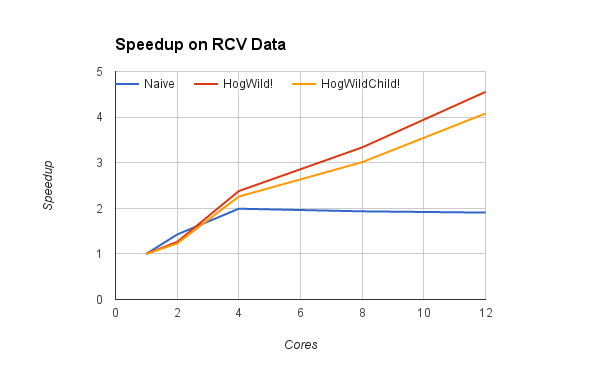
\includegraphics[width=\textwidth]{img/rcv_graph.png}
\label{rcv}
\caption{Graph of speedup on the RCV data}
\end{figure}

We also note that our HogWildChild! implementation is slightly slower
than the regular HogWild!, and that WildChild! does not improve the
error rates on a 12-threaded program.

On this dataset, 0.3\% of decision variables met the $\rfrac 1 p$
threshold for being stashed in a pending changes \texttt{UpdateVector},
with a total of 27.9\% of accesses meeting this threshold.
i.e, Even though only 0.3\% of decision variables met the threshold,
these variables occur frequently enough that they make up
27.9\% of decision variables used across all training samples.

\subsection{Wikipedia Data}

The Wikipedia dataset consists of approximately 120,000 training samples
and 10,000 testing samples.
We made this dataset by downloading Wikipedia's database in German and
Portuguese, and converting articles into the 3-grams therein.
As shown in Table \ref{tab-wiki}, just by looking at the 3-grams we were
able to determine language with approximately 98\% accuracy.

\begin{table}[h!]
\centering
\begin{tabular}{| c | c | c | c |}
\hline
Threads & Naive	(s)	& HogWild! (s)	& HogWildChild! (s) \\
\hline
1	& 9.51		& ---		& --- 	\\
2	& 5.31		& 5.56		& 5.72	\\
4	& 3.31		& 2.94		& 3.13	\\
8	& 2.57		& 2.20		& 2.50	\\
12	& 2.22		& 1.63		& 1.88	\\
\hline
Train Error (12 thread) & 1.96\%	& 1.96\%	& 1.98\% \\
Test Error  (12 thread) & 2.21\%	& 2.18\%	& 2.24\% \\
\hline
\end{tabular}
\label{tab-wiki}
\caption{Table of the execution times for 20 epochs of the Wikipedia data}
\end{table}

As in the RCV dataset, we were easily able to achieve the targeted 4x
speedup over the serial approach.

In this dataset, we see that the Naive approach does not plateau nearly
as dramatically as in the RCV data.
This is likely because samples in our Wiki dataset were smaller than in the
RCV dataset, and so required holding the lock for less time.

\begin{figure}[h!]
\centering
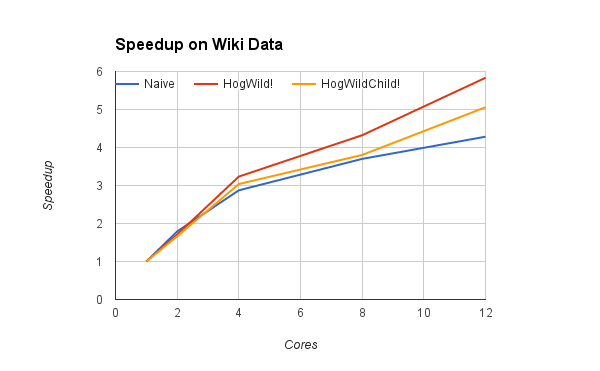
\includegraphics[width=\textwidth]{img/wiki_graph.png}
\label{wiki}
\caption{Graph of speedup on the Wikipedia language recognizer}
\end{figure}

Further, the HogWildChild! implementation is still slower than HogWild!,
and no more accurate.
On this dataset, 0.23\% of decision variables pass the $\rfrac 1 p$
threshold on 12 threads.
However, 39.81\% of decision variables used across all training samples
pass by this threshold.
This means that 40\% of the time, when updating a decision variable it's
likely that another thread is currently using the same variable.

\subsection{HogWildChild! and Error Rates}

Our goal with HogWildChild! was to come up with an approach which better
dealt with frequent variables than the HogWild algorithm.
However, we saw that the HogWild! algorithm achieved the same error on
both of our datasets as the serial algorithm.
As such, we were unable to come up with a parallel algorithm that could
actually achieve better accuracy than HogWild!, and we were surprised by
how well HogWild! performed even when 40\% of the variables used occured
over the $\rfrac 1 p$ threshold.

\subsection{Breaking Point}

HogWildChild! uses a $\rfrac 1 p$ threshold to determine which decision
variables should have changes stashed until sufficiently many changes had
been seen.
As such, increasing the number of threads will increase the percentage of
decision variables which are over the threshold.
The unix.andrew.cmu.edu machines have 20 cores, with up to 40 processes
hyperthreaded.
When run on the RCV data, we see:

\begin{figure}[h!]
\centering
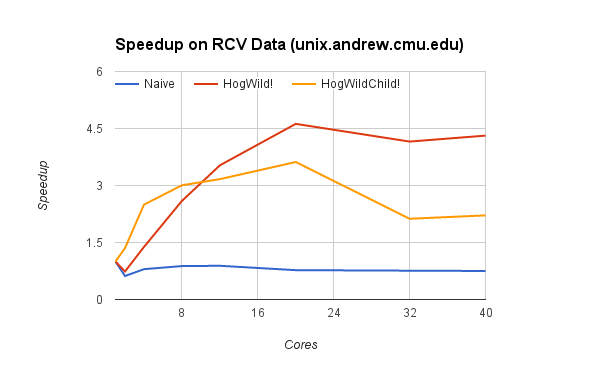
\includegraphics[width=\textwidth]{img/unix_graph.png}
\label{unix-rcv}
\caption{Graph of speedup on the Wikipedia language recognizer}
\end{figure}

In the 40-threaded run on the RCV data, the 1.4\% of decision variables
above the $\rfrac 1 p$ threshold accounted for nearly 60\%
the decision variables used.
Further, since the threshold is so much smaller, decision variables need to
stay in the \texttt{UpdateVector} until they've witnessed more changes.
This accounts for the serious slow-down of HogWildChild! around 20 threads.

\begin{figure}[h!]
\centering
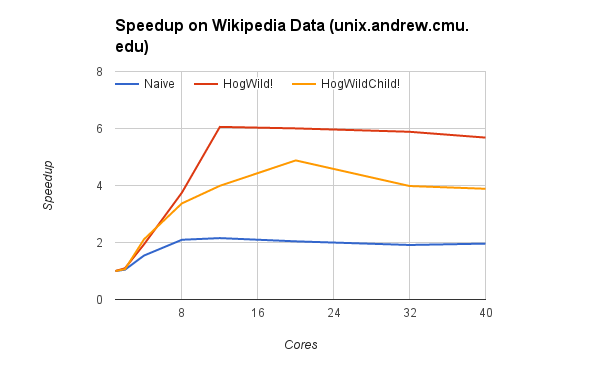
\includegraphics[width=\textwidth]{img/unix_wiki_graph.png}
\label{unix-wiki}
\caption{Graph of speedup on the Wikipedia language recognizer}
\end{figure}

Figure \ref{unix-wiki} shows a similar result, with HogWildChild!
slowing down after 20 threads.
At 40 threads, 64\% of decision variables used are above the
$\rfrac 1 p$ frequency threshold.

Interestingly, Figure \ref{unix-wiki} shows HogWild! plateauing around 12
threads.
This is likely due to the memory bandwidth constraints,
as at this point HogWild! is reading and writing faster than
unix.andrew.cmu.edu's memory bus can deal with.

\section{Work Performed By Student}

Equal work was performed by both project members.

\clearpage
\addcontentsline{toc}{section}{References}
\begin{thebibliography}{9}
\bibitem{hogwild}
Feng Niu, Benjamin Recht, Christopher R\'e, and Stephen J. Wright.
\emph{HogWild!: A Lock-Free Approach to
Parallelizing Stochastic Gradient Descent},
Computer Sciences Department, University of Wisconsin-Madison,
2011.
\texttt{http://www.eecs.berkeley.edu/$\sim$brecht/papers/hogwildTR.pdf}
\end{thebibliography}

\end{document}
